\documentclass[a4paper, 12pt]{article}
\usepackage[a4paper,top=1.5cm, bottom=1.5cm, left=1cm, right=1cm]{geometry}
\usepackage{cmap}					
\usepackage{mathtext} 				
\usepackage[T2A]{fontenc}			
\usepackage[utf8]{inputenc}			
\usepackage[english,russian]{babel}
\usepackage{multirow}
\usepackage{graphicx}
\usepackage{wrapfig}
\usepackage{tabularx}
\usepackage{float}
\usepackage{longtable}
\usepackage{hyperref}
\hypersetup{colorlinks=true,urlcolor=blue}
\usepackage[rgb]{xcolor}
\usepackage{amsmath,amsfonts,amssymb,amsthm,mathtools} 
\usepackage{icomma} 
\usepackage{euscript}
\usepackage{mathrsfs}
\usepackage{enumerate}
\usepackage{caption}
\usepackage{enumerate}
\mathtoolsset{showonlyrefs=true}
\usepackage{graphicx}
\usepackage{caption}
\usepackage{subcaption}
\usepackage{amsthm}
\usepackage[europeanresistors, americaninductors]{circuitikz}
\DeclareMathOperator{\sgn}{\mathop{sgn}}
\newcommand*{\hm}[1]{#1\nobreak\discretionary{}
	{\hbox{$\mathsurround=0pt #1$}}{}}

%%% Заголовок

\title{\textbf{Эффект Джоуля-Томсона (2.1.6)}}
\author{Манро Эйден}
\date{}

\begin{document}

\maketitle

\begin{center}
    \section*{Введение}
\end{center}

\noindent \textbf{Цель работы:} 1) Определение изменения температуры углекислого газа при протекании через малопроницаемую перегородку при разных начальных значениях давления и температуры; 2) вычисление по результатам опытов коэффициентов Ван-дер-Ваальса <<a>> и <<b>>.

\bigskip

\noindent \textbf{Оборудование:} трубка с пористой перегородкой; труба Дьюара; термостат; термометры; дифференциальная термопара; микровольтметр; балластный баллон; манометр.

\bigskip

Эффектом Джоуля–Томсона называется изменение температуры газа, медленно протекающего из области высокого в область низкого давления в условиях хорошей тепловой изоляции. В разреженных газах, которые приближаются по своим свойствам к идеальному газу, при таком течении температура газа не меняется. Эффект Джоуля–Томсона демонстрирует отличие исследуемого газа от идеального.
	
	В работе исследуется изменение температуры углекислого газа при медленном его течении по трубке с пористой перегородкой. Трубка 1 хорошо теплоизолирована. Газ из области повышенного давления $P_1$ проходит через множество узких и длинных каналов пористой перегородки 2 в область с атмосферным давлением $P_2$. Перепад давления  $\Delta P = P_1 - P_2$ из-за большого сопротивления каналов может быть заметным даже при малой скорости течения газа в трубке. Величина эффекта Джоуля–Томсона определяется по разности температуры газа до и после перегородки.
	
	Рассмотрим стационарный поток газа между произвольными сечениями I и II трубки (до перегородки и после нее). Пусть, для определенности, через трубку прошел 1 моль углекислого газа; $\mu$ — его молярная масса. Молярные объемы газа, его давления и отнесенные к молю внутренние энергии газа в сечениях I и II обозначим соответственно $V_1$, $P_1$, $U_1$ и $V_2$ , $P_2$ , $U_2$. Для того чтобы ввести в трубку объем $V_1$, над газом нужно совершить работу $A_1$ = $P_1 V_1$. Проходя через сечение II, газ сам совершает работу $A_2$ = $P_2$ $V_2$. Так как через боковые стенки не происходит ни обмена теплом, ни передачи механической энергии, то
	\begin{equation}
		A_1-A_2 = \left(U_2+\frac{\mu v_2^2}{2}\right)-\left(U_1+\frac{\mu v_1^2}{2}\right).
	\end{equation}
	В уравнении (1) учтено изменение как внутренней (первые члены в скобках), так и кинетической (вторые члены в скобках) энергии газа. Подставляя в (1) написанные выражения для $A_1$ и $A_2$ и перегруппировывая члены, найдем
	\begin{equation}
		H_1-H_2 = \left(U + P_1 V_1 \right) - \left(U_2 + P_2 V_2 \right) = \frac{1}{2}\mu\left(v_2^2-v_1^2\right)
	\end{equation}
	
	Сделаем несколько замечаний. Прежде всего отметим, что в процессе Джоуля–Томсона газ испытывает в пористой перегородке существенное трение, приводящее к ее нагреву. Потери энергии на нагрев трубки в начале процесса могут быть очень существенными и сильно искажают ход явления. После того как температура трубки установится и газ станет уносить с собой все выделенное им в пробке тепло, формула (1) становится точной, если, конечно, теплоизоляция трубки достаточно хороша и не происходит утечек тепла наружу через ее стенки.
	
	Второе замечание связано с правой частью (2). Процесс Джоуля–Томсона в чистом виде осуществляется лишь в том случае, если правой частью можно пренебречь, т. е. если макроскопическая скорость газа с обеих сторон трубки достаточно мала. У нас сейчас нет критерия, который позволил бы установить, когда это можно сделать. Поэтому мы отложим на некоторое время обсуждение вопроса о правой части (2), а пока будем считать, что энтальпия газа не меняется.
	
	Рассмотрим выражение:
	\begin{equation}
		\mu_{\text{Д-Т}} = \frac{\Delta T}{\Delta P} \approx \cfrac{\cfrac{2a}{RT}-b}{C_p}
	\end{equation}
	
	Из формулы (3) видно, что эффект Джоуля–Томсона для не очень плотного газа зависит от соотношения величин $a$ и $b$, которые оказывают противоположное влияние на знак эффекта. Если силы взаимодействия между молекулами велики, так что превалирует «поправка на давление», то основную роль играет член, содержащий $a$, и
	\[ \frac{\Delta T}{\Delta P} > 0, \]
	то есть газ при расширении охлаждается ($\Delta t < 0$ так как всегда
	$\Delta P < 0$). В обратном случае (малые a):
	\[ \frac{\Delta T}{\Delta P} < 0, \]
	то есть газ нагревается ($\Delta t < 0$ так как по-прежнему $\Delta P < 0$).
	
	Этот результат нетрудно понять из энергетических соображений. Как мы уже знаем, у идеального газа эффект Джоуля–Томсона отсутствует. Идеальный газ отличается от реального тем, что в нем можно пренебречь потенциальной энергией взаимодействия молекул. Наличие этой энергии приводит к охлаждению или нагреванию реальных газов при расширении. При больших $a$ велика энергия притяжения молекул. Это означает, что потенциальная энергия молекул при их сближении уменьшается, а при удалении — при расширении газа -- возрастает. Возрастание потенциальной энергии молекул происходит за счет их кинетической энергии -- температура газа при расширении падает. Аналогичные рассуждения позволяют понять, почему расширяющийся газ нагревается при больших значениях $b$.
	
	Как следует из формул, при температуре $T_i$ коэффициент $\mu_\text{д-т}$ обращается в нуль. Используя связь между коэффициентами $a$ и $b$ и критической температурой, найдем:
	\begin{equation}
		T_{инв}=\frac{2a}{bR}, \qquad
		T_{инв}=\frac{27}{4}T_{кр}
	\end{equation}
	
	При температуре $T_\text{инв}$ эффект Джоуля–Томсона меняет знак: ниже температуры инверсии эффект положителен ($\mu_\text{д-т} > 0$, газ охлаждается), выше $T_\text{инв}$ эффект отрицателен ($\mu_\text{д-т} < 0$, газ нагревается).	
	
	
	\begin{figure}[h!]
		\centering{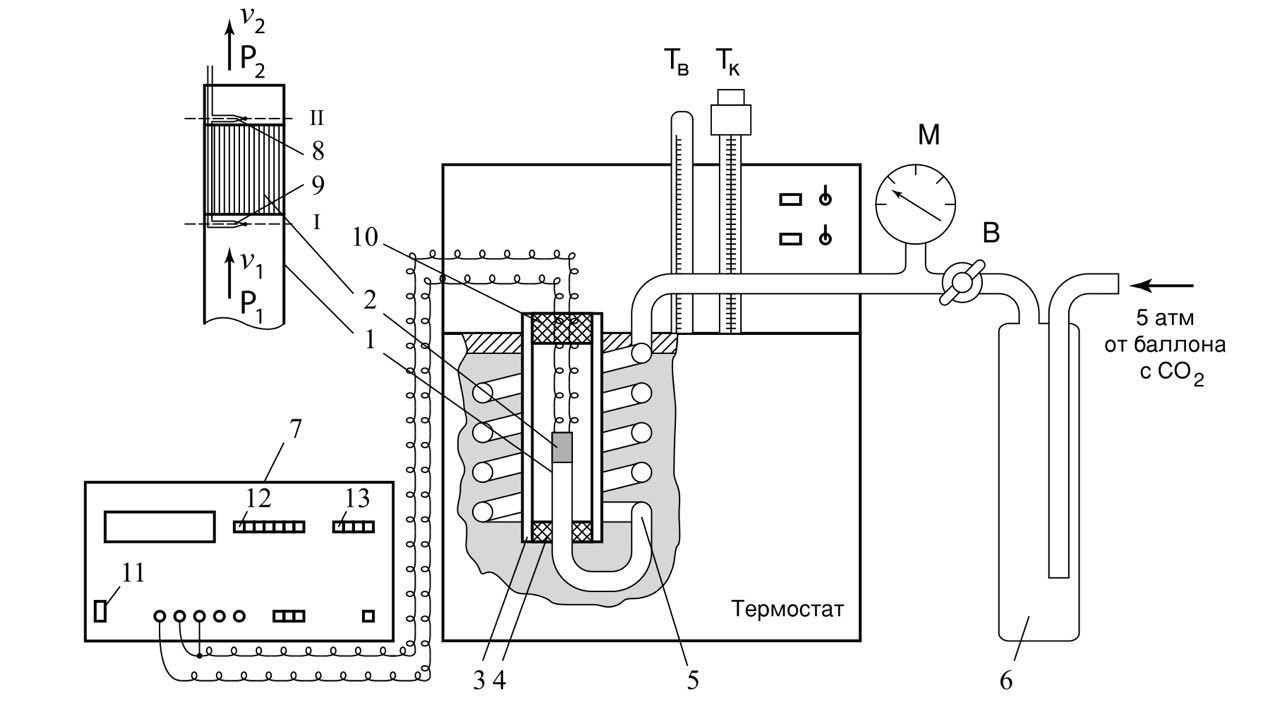
\includegraphics[width=0.75\textwidth]{ust.jpg}}
		\caption[]{\label{fig:1} Схема установки для изучения эффекта Джоуля–Томсона}
	\end{figure}

\end{document}